%% This is file `elsarticle-template-1-num.tex',
%%
%% Copyright 2009 Elsevier Ltd
%%
%% This file is part of the 'Elsarticle Bundle'.
%% ---------------------------------------------
%%
%% It may be distributed under the conditions of the LaTeX Project Public
%% License, either version 1.2 of this license or (at your option) any
%% later version.  The latest version of this license is in
%%    http://www.latex-project.org/lppl.txt
%% and version 1.2 or later is part of all distributions of LaTeX
%% version 1999/12/01 or later.
%%
%% Template article for Elsevier's document class `elsarticle'
%% with numbered style bibliographic references
%%
%% $Id: elsarticle-template-1-num.tex 149 2009-10-08 05:01:15Z rishi $
%% $URL: http://lenova.river-valley.com/svn/elsbst/trunk/elsarticle-template-1-num.tex $
%%
\documentclass[preprint,12pt]{elsarticle}

%% Use the option review to obtain double line spacing
%% \documentclass[preprint,review,12pt]{elsarticle}

%% Use the options 1p,twocolumn; 3p; 3p,twocolumn; 5p; or 5p,twocolumn
%% for a journal layout:
%% \documentclass[final,1p,times]{elsarticle}
%% \documentclass[final,1p,times,twocolumn]{elsarticle}
%% \documentclass[final,3p,times]{elsarticle}
%% \documentclass[final,3p,times,twocolumn]{elsarticle}
%% \documentclass[final,5p,times]{elsarticle}
%% \documentclass[final,5p,times,twocolumn]{elsarticle}

%% The graphicx package provides the includegraphics command.
\usepackage{graphicx}
%% The amssymb package provides various useful mathematical symbols
\usepackage{amssymb}
%% The amsthm package provides extended theorem environments
%% \usepackage{amsthm}

%% The lineno packages adds line numbers. Start line numbering with
%% \begin{linenumbers}, end it with \end{linenumbers}. Or switch it on
%% for the whole article with \linenumbers after \end{frontmatter}.
\usepackage{lineno}


%% natbib.sty is loaded by default. However, natbib options can be
%% provided with \biboptions{...} command. Following options are
%% valid:

%%   round  -  round parentheses are used (default)
%%   square -  square brackets are used   [option]
%%   curly  -  curly braces are used      {option}
%%   angle  -  angle brackets are used    <option>
%%   semicolon  -  multiple citations separated by semi-colon
%%   colon  - same as semicolon, an earlier confusion
%%   comma  -  separated by comma
%%   numbers-  selects numerical citations
%%   super  -  numerical citations as superscripts
%%   sort   -  sorts multiple citations according to order in ref. list
%%   sort&compress   -  like sort, but also compresses numerical citations
%%   compress - compresses without sorting
%%
%% \biboptions{comma,round}

% \biboptions{}

\journal{Journal Name}

\usepackage[top=1in, bottom=1.5in, left=1in, right=1in]{geometry}
\usepackage[
    %backend=biber, 
    natbib=true,
    style=numeric,
    sorting=none
]{biblatex}
\addbibresource{sample.bib}

\begin{document}


%\begin{frontmatter}

%% Title, authors and addresses

%\title{b~flavored Jets as a Handle for Direct Measurement of ggH production of the Higgs and its subsequent decay to $b\bar{b}$ during Run 3 and Run 4 at the LHC/HL-LHC}

%% use the tnoteref command within \title for footnotes;
%% use the tnotetext command for the associated footnote;
%% use the fnref command within \auth or or \address for footnotes;
%% use the fntext command for the associated footnote;
%% use the corref command within \author for corresponding author footnotes;
%% use the cortext command for the associated footnote;
%% use the ead command for the email address,
%% and the form \ead[url] for the home page:
%%
%% \title{Title\tnoteref{label1}}
%% \tnotetext[label1]{}
 %\author{Prof. Isobel Ojalvo}
 %\ead{iojalvo@princeton.edu}
%% \ead[url]{home page}
%% \fntext[label2]{}
%% \cortext[cor1]{}
%% \address{Address\fnref{label3}}
%% \fntext[label3]{}


%% use optional labels to link authors explicitly to addresses:
%% \author[label1,label2]{<author name>}
%% \address[label1]{<address>}
%% \address[label2]{<address>}

%\author{John Smith}

%\address{California, United States}

%\begin{abstract}
%% Text of abstract
%Suspendisse potenti. Suspendisse quis sem elit, et mattis nisl. Phasellus consequat erat eu velit rhoncus non pharetra neque auctor. Phasellus eu lacus quam. Ut ipsum dolor, euismod aliquam congue sed, lobortis et orci. Mauris eget velit id arcu ultricies auctor in eget dolor. Pellentesque suscipit adipiscing sem, imperdiet laoreet dolor elementum ut. Mauris condimentum est sed velit lacinia placerat. Vestibulum ante ipsum primis in faucibus orci luctus et ultrices posuere cubilia Curae; Nullam diam metus, pharetra vitae euismod sed, placerat ultrices eros. Aliquam tincidunt dapibus venenatis. In interdum tellus nec justo accumsan aliquam. Nulla sit amet massa augue.
%\end{abstract}


%\begin{keyword}
%Science \sep Publication \sep Complicated
%% keywords here, in the form: keyword \sep keyword

%% MSC codes here, in the form: \MSC code \sep code
%% or \MSC[2008] code \sep code (2000 is the default)

%\end{keyword}

%\end{frontmatter}

%%
%% Start line numbering here if you want
%%
%\linenumbers

%% main text


\noindent
\textbf{Using Tau Leptons as a Tool for Studying the Higgs in the SM and Beyond}

\section{Overview}
As a member of the Compact Muon Solenoid (CMS) experiment~\cite{CMS-JINST} at the LHC, 
I propose to introduce novel methods to the current and future online CMS trigger systems 
in order to improve the identification and acquisition of events containing rare physics. 
With the arrival of new high-level synthesis technologies that allow engineers and 
physicists to quickly and easily translate advanced algorithms into hardware 
description language, it is possible to target specific Standard Model Higgs
production mechanisms at the event level. We are developing event-level triggers 
to identify events that contain two back-to-back quark jets, indicative of 
Vector Boson Fusion, a single fat jet with sub-structure, indicative of a boosted
object topology. %Or a an anomaly based trigger... finish me.

I am currently leading the CMS physics analysis in the characterization of the Higgs 
Boson in its decay to tau ($\tau$) leptons with the full Run 2 dataset; previously as 
a postdoc I led the analysis effort which resulted in the first observation of the 
Higgs in its decay to taus by a single experiment~\cite{HIG16043}. This observation was the 
result of iterative development and improvements to the $\tau$ trigger, reconstruction 
and identification by the CMS collaboration. I have contributed to these efforts and served 
in leadership positions in the CMS collaboration first as the developer of the Level-1 
trigger $\tau$ algorithm, put into place in 2015, then as the convener of the tau trigger
development group (2014-2015) and later as the convener of the tau physics object group 
(2015-2018). Currently, I serve as the US CMS Level-1 Trigger Operations deputy. 
As a new faculty member at Princeton, I have used my startup funding to hire an 
engineer, Luis Perez Moreno, who is working on CMS Level-1 Trigger firmware development
for Run 3 and Run 4 with the US APD hardware consortium. He is supporting operations 
of the calorimeter trigger at 
CMS and will work with postdoc, Pallabi Das, and graduate student, Stephanie Kwan, on
implementation of these event-based algorithms. Based upon our first developments of
this project, Stephanie Kwan, has received the NSF graduate student research award
and her tuition and salary is supported by the NSF. She and Pallabi Das are stationed
at CERN, supporting CMS Level-1 trigger operations, their cost of living is supported 
through detector operations.

My group's primary physics activities are the precision measurements of the electroweak symmetry breaking mechanism, 
precision measurements of the the Higgs Yukawa coupling and searches for associated new physics phenomena. 
The observation of the Higgs in its decay to taus by the CMS experiment in 2017 sets the context for my 
current and future research program. It strengthens the case for using the Higgs in its decay to taus for 
detailed study of the properties of this new boson. 
This physics process will also be leveraged in searches for beyond the standard model supersymmetric Higgs bosons. 

\section{Proposed Research Direction}

The basic framework of the Standard Model (SM) works for many particle physics interactions and 
measurements but is not an all-encompassing theory; many questions still remain. The visible 
universe---stars, planets, the Earth---are composed of matter due to a tiny difference in behavior 
of anti-matter versus matter, but the SM has no good explanation for this phenomenon. %Equally important, cosmological studies indicate that 84.5 percent of the matter in the universe is composed of some sort of ’dark matter’ that can exert a gravitational force and yet does not interact via the Standard Model mechanisms. 
After the discovery of the Higgs boson in Run 1, the primary mission of the LHC in Run 2 is 
the search for new physics. This includes exploring possible unification of forces, resolving the hierarchy problem 
and understanding the nature of dark matter and requires a 
deep understanding of the Higgs boson characteristics, as any deviations from perfect SM 
behavior due to anomalous particles could lead to deeper understanding of the fundamental particle 
interactions~\cite{Curtin:2013fra}. My group plans to continue its study of the SM Higgs 
boson and search for new Higgs bosons. 

\subsection{SM Higgs decays to $\tau$ pairs}
In the SM, the mass generation of fermions is achieved through the Higgs Yukawa coupling~\cite{Higgs:1966ev,Denner:2011mq}.
There exists several more fundamental theories, such as supersymmetry, %~cite
that could imply deviations of the couplings of the observed Higgs boson to down-type fermions, such as
the $\tau$ lepton. Therefore, it is necessary to demonstrate the direct coupling of the Higgs boson to the fundamental fermions and to demonstrate
the proportionality of the Higgs boson coupling strength to their mass. 
The most promising decay channel in which to do this is 
$\tau\tau$ due to the large expected event rate when compared to the $\mu^{+}\mu^{-}$ 
channel and smaller contribution from background events with respect to the $bb$ channel.

The first observation of $H\rightarrow \tau \tau$ with a single experiment was performed 
at CMS using data from Run 1 and 35.9 fb$^{-1}$ from the 2016 data set~\cite{Aad:2015vsa}. 
In this analysis all possible $\tau\tau$ final states are considered except for those with
two electrons or two muons due to the low branching fraction and large background 
contribution of those two channels. The event sample is split into three mutually exclusive categories
per final state. In each category the two variables that maximize the $H\rightarrow \tau \tau$ 
discovery potential are chosen to build two-dimensional (2D) distributions. The 
categories are defined as 0-jet, which serves as a control region due to its low signal
efficiency, VBF, which targets Higgs events produced via Vector Boson Fusion (VBF), and
Boosted, which targets Higgs boson events produced via gluon fusion (ggH). The observed and predicted 2D distribution
in the VBF category of the $\tau_{h}\tau_{h}$ final state can be seen in Fig.~\ref{fig:vbf_2016}.
The combination with the corresponding searches using data collected by the CMS experiment 
at center-of-mass energies of 7 and 8~TeV lead to an observed significance of 5.9 standard 
deviations, equal to the expected significance. In comparison with $\gamma\gamma$, ZZ, WW, 
bb and $\mu\mu$, the $\tau\tau$ final state provides the most stringent measurement of the 
VBF production mechanism~\cite{Sirunyan:2018koj}; this is seen in Fig.~\ref{fig:Sirunyan2018koj}.
%check building
\begin{figure*}[htbp]
\centering
     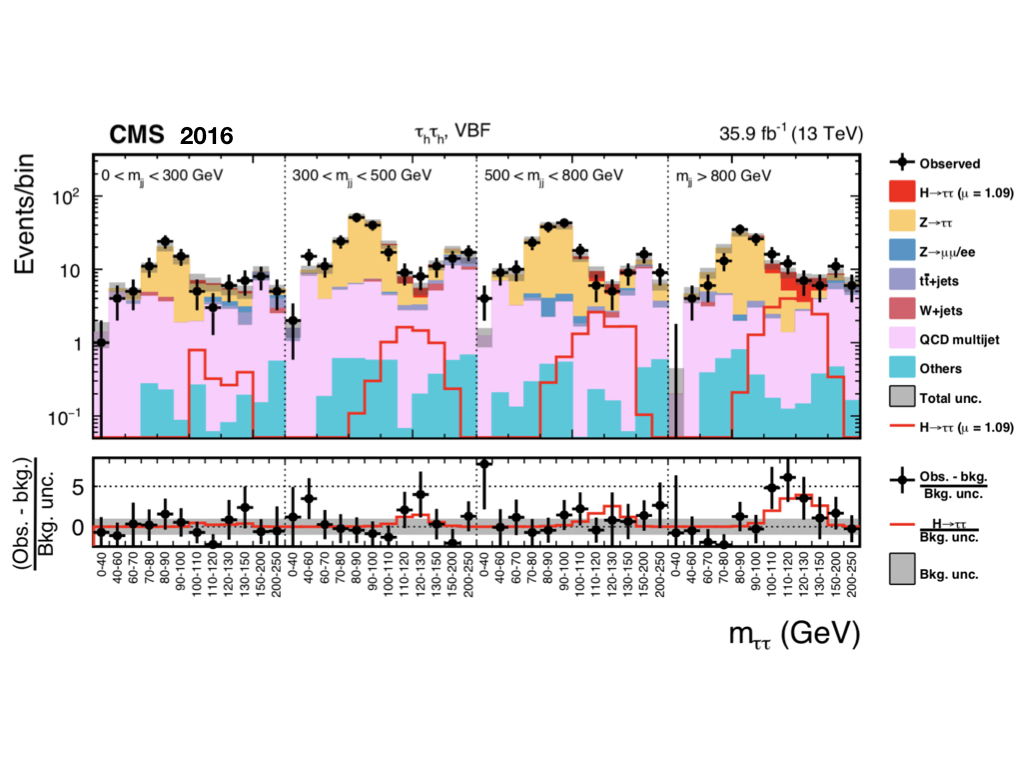
\includegraphics[trim=0 120 0 120,clip,width=0.75\textwidth]{HTT_Plots_2016.jpeg}
     \caption{Observed and predicted 2D distributions in the VBF category of the $\tau_{h}\tau_{h}$ channel from the public 2016 analysis. The bins are unrolled in $m_{jj}$ with slices corresponding to $m_{jj} = [0,350,500,800,+]$.}
     \label{fig:vbf_2016}
\end{figure*}

\begin{figure}[h]
\centering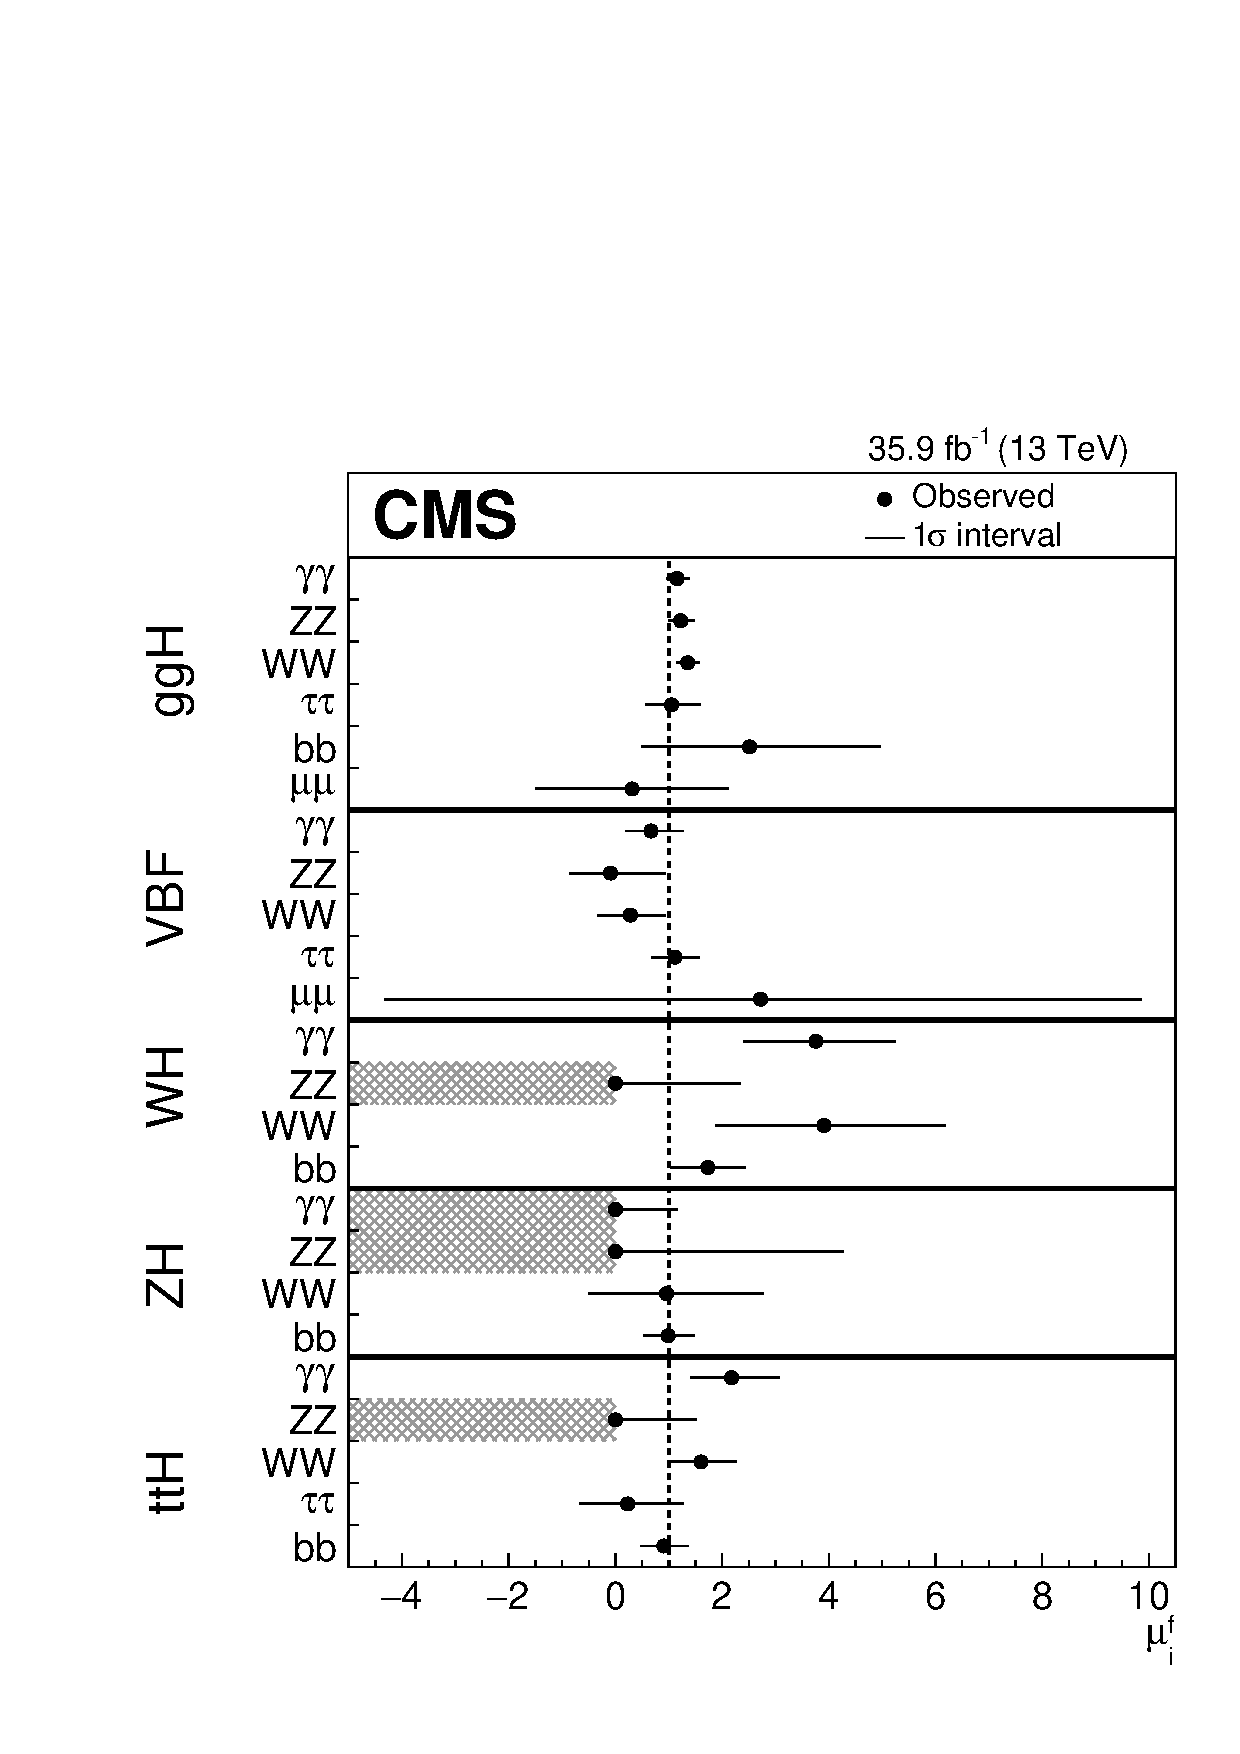
\includegraphics[width=0.4\linewidth]{CMS-HIG-17-031_Figure_006_VBF_Comparison.pdf}
\caption{In comparison with $\gamma\gamma$, ZZ, WW, bb and $\mu\mu$, the $\tau\tau$ final state provides the most stringent measurement of the VBF production mechanism~\cite{Sirunyan:2018koj} at CMS.}
\label{fig:Sirunyan2018koj}
\end{figure}

%%proposed research direction
We are focusing our efforts on three areas for improvement: Vector Boson Fusion  identification, Boosted Jet Substructure, and Long Lived Particle identification

Higgs to Tau Tau VBF – efficiency, rate
Higgs to Tau Tau ggH Boosted – efficiency, rate
Higgs to Tau Tau + b-tagging – efficiency, rate


VBF production cross section - as compared to ggH
By implementing a VBF only based trigger other channels will also be able
to leverage this as a mechanism for XX, in particular, the Higgs it can be
used to detect Higgs in its decay to Dark Matter (higgs to invisible)

LLP


\newpage
%% The Appendices part is started with the command \appendix;
%% appendix sections are then done as normal sections
%% \appendix

%% \section{}
%% \label{}

%% References
%%
%% Following citation commands can be used in the body text:
%% Usage of \cite is as follows:
%%   \cite{key}          ==>>  [#]
%%   \cite[chap. 2]{key} ==>>  [#, chap. 2]
%%   \citet{key}         ==>>  Author [#]

%% References with bibTeX database:

%\bibliographystyle{model1-num-names}

%\bibliography{sample.bib}
\printbibliography

%% Authors are advised to submit their bibtex database files. They are
%% requested to list a bibtex style file in the manuscript if they do
%% not want to use model1-num-names.bst.

%% References without bibTeX database:

% \begin{thebibliography}{00}

%% \bibitem must have the following form:
%%   \bibitem{key}...
%%

% \bibitem{}

% \end{thebibliography}


\end{document}

%%
%% End of file `elsarticle-template-1-num.tex'.
